\subsection{Cluster Analysis Results Visualization}
\label{sec:cluster}

The Figure~\ref{fig:Cytoscape_Cluster_2} from Section~\ref{sec:dataset_description} shows cluster graph specific structure: it is very high, unbalanced and has not so deep sub-parts. It is possible to use this disadvantage as advantage and abstract sub-parts to reduce drawing area. Extract those nodes and edges that form the longest path of the cluster graph - ,,backbone''. Figure~\ref{fig:cluster_visualisation} shows algorithm work step by step. Backbone vertices are filled with yellow and showed on the Figure~\ref{fig:cluster_visualisation_algorithm_1}. Next step is to abstract branches into groups, group size is scaled according to amount of elements inside.

\begin{figure}[h!]
\centering
\subfloat[Backbone and branches]{
    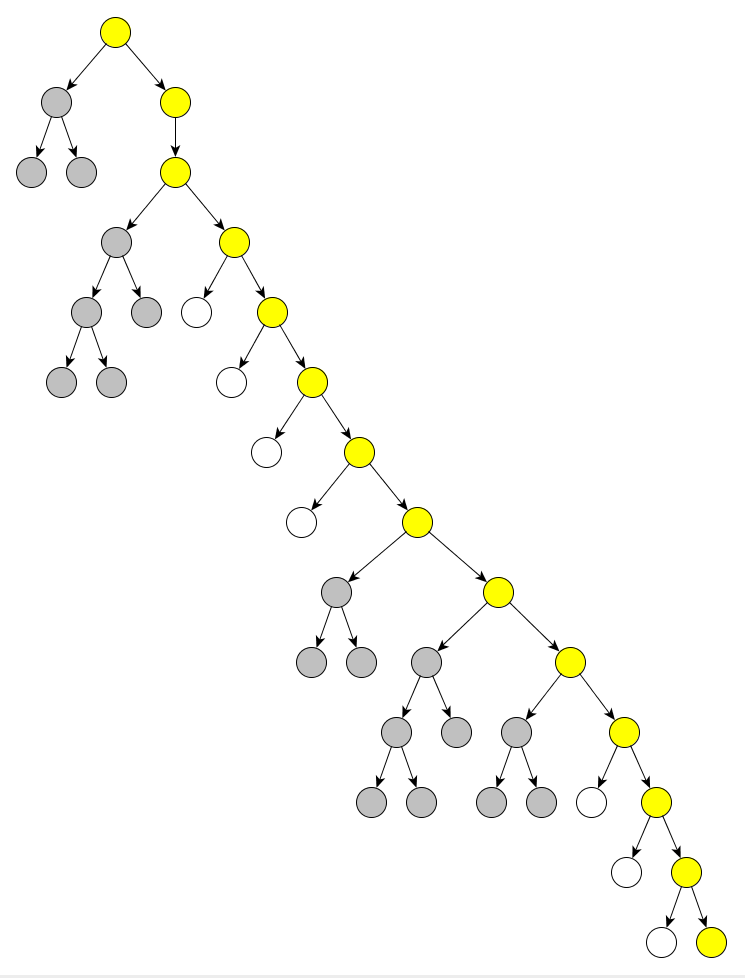
\includegraphics[scale=0.15]{pictures/cluster_visualisation_algorithm_1.png}
    \label{fig:cluster_visualisation_algorithm_1}
}
\subfloat[Abstract branches into groups]{
    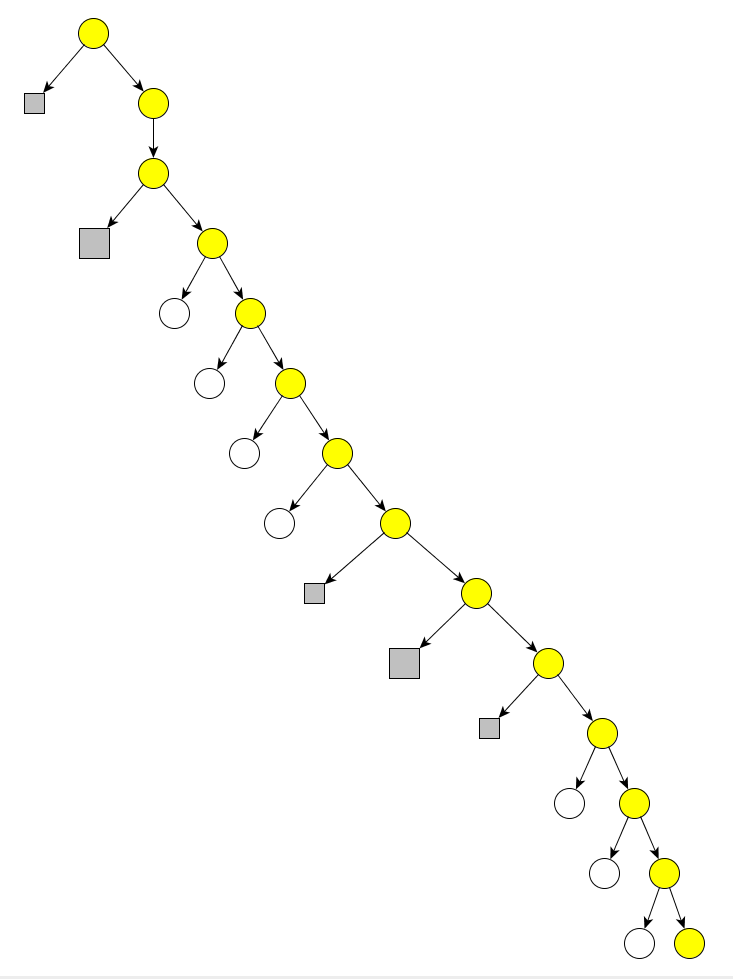
\includegraphics[scale=0.15]{pictures/cluster_visualisation_algorithm_2.png}
    \label{fig:cluster_visualisation_algorithm_2}
}
\subfloat[Scale group size]{
    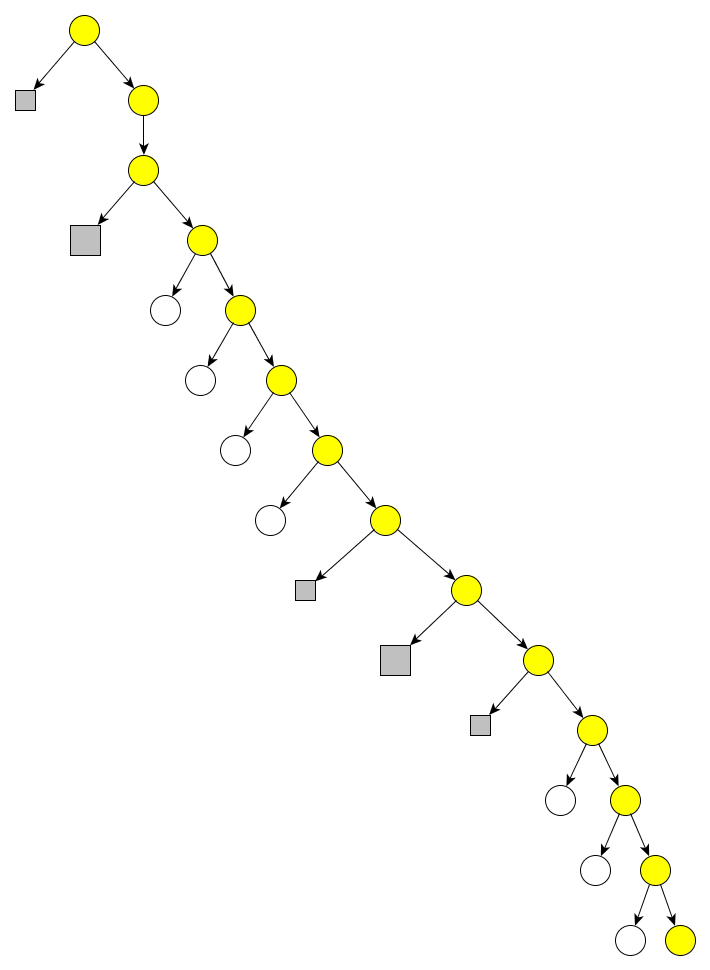
\includegraphics[scale=0.15]{pictures/cluster_visualisation_algorithm_3.png}
    \label{fig:cluster_visualisation_algorithm_3}
}
\caption{Cluster Visualization algorithm}
\label{fig:cluster_visualisation_algorithm}
\end{figure}

The last step is to represent backbone as a spiral, thus preserving space and giving us a possibility to show the complete tree in one view. Figure~\ref{fig:cluster_visualisation_algorithm_4} shows how this approach works.

\begin{figure}[h!]
\centering
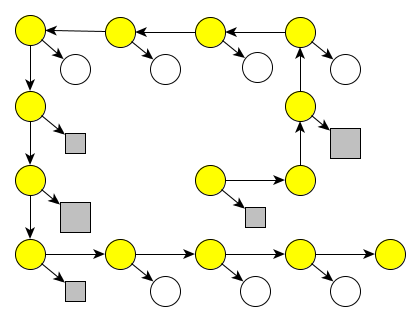
\includegraphics[scale=0.5]{pictures/cluster_visualisation_algorithm_4.png}
\caption{,,Rectangular Spiral Layout''}
\label{fig:cluster_visualisation_algorithm_4}
\end{figure}

Then backbone formed as rectangular spiral with a root in the center and moving in clockwise direction. Figure~\ref{fig:cluster_spiral_visualisation} shows complete visualisation result for real cluster tree. This will have to reuse space as much as possible and still gives overview of location of the highlighted vertices in cluster hierarchy -- how far from a root.

\begin{figure}[h!]
\centering
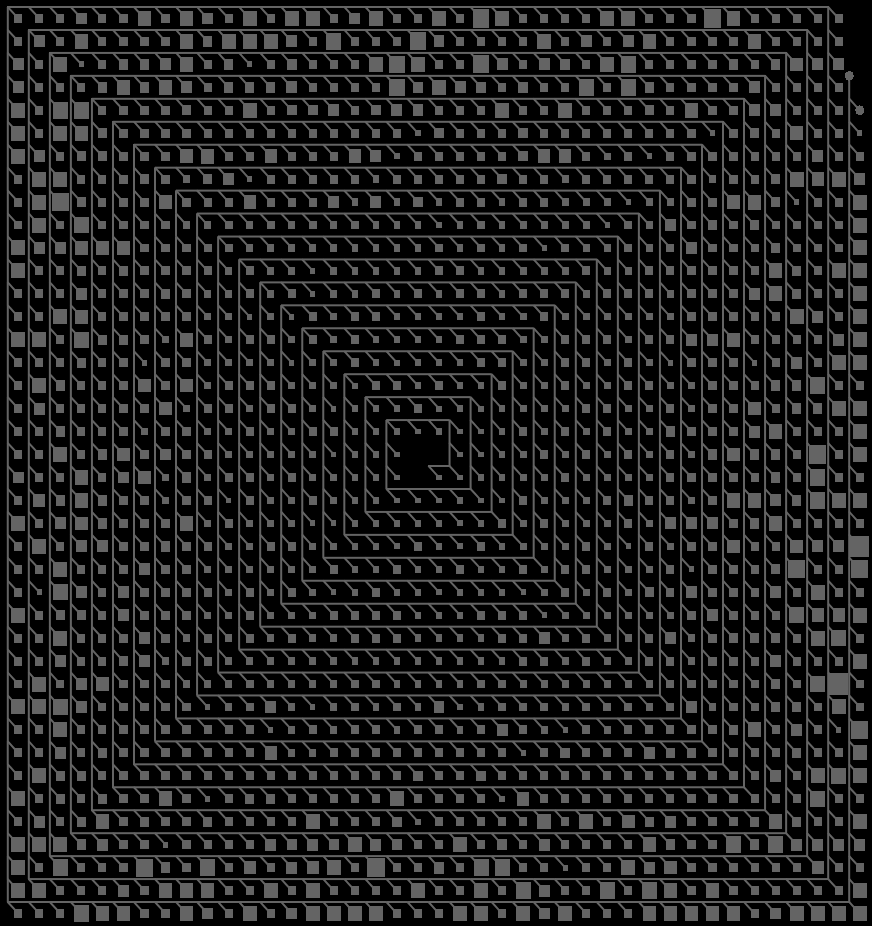
\includegraphics[scale=0.4]{pictures/cluster_spiral_visualisation.png}
\caption{Rectangular spiral Cluster graph visualisation}
\label{fig:cluster_visualisation}
\end{figure}

It is possible to explore sub-part (rectangles) of the Cluster graph using lens. User can interactively choose any sub-part and lens with inned content will appear. There are two different lens layouts: polar~\ref{fig:lens_polar} and HV-tree~\ref{fig:lens_tree}. Polar lens layout is based on Both implementations are own implementations and are not depend of any external library.

\begin{figure}[h!]
\centering
\subfloat[Polar lens layout]{
    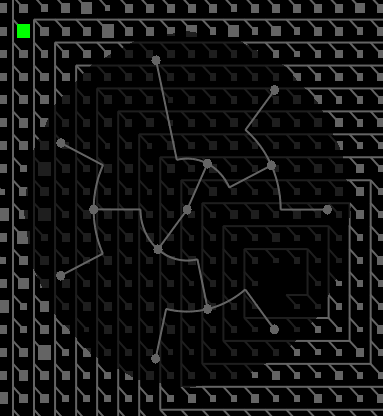
\includegraphics[scale=0.5]{pictures/lens_polar.png}
    \label{fig:lens_polar}
}
\\
\subfloat[HV-tree lens layout]{
    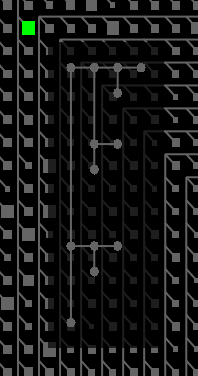
\includegraphics[scale=0.5]{pictures/lens_tree.png}
    \label{fig:lens_tree}
}
\caption{Different lens layouts}
\end{figure}

